Recall that for each  the number of \ktypes is finite. Let  be this
number. Proposition~\ref{prop-nec-implies-LT} is an immediate consequence of
the following proposition.

\begin{prop}\label{lemma-pumping}
  Let  be a \ktame regular tree language. Set .
  Then for all  and any two trees  if
  \sameblocks{t}{t'}{\kappa} then there exist two trees  with
\begin{enumerate}[\em(1)]
\item  ~iff~ 
\item  ~iff~ 
\item \sameblocks{T}{T'}{l}
\end{enumerate}
\end{prop}

\begin{proof}[Proof of Proposition~\ref{prop-nec-implies-LT} using
  Proposition~\ref{lemma-pumping}]
  Assume  is \ktame and let  be defined as in
  Proposition~\ref{lemma-pumping}. We show that  is in LT iff  is
  \testable{\kappa}. Assume  is in LT. Then  is \testable{l} for some . We show that  is actually \testable{\kappa}. For this it
  suffices to show that for any pair of trees  and , if
  \sameblocks{t}{t'}{\kappa} then  iff . Let  and  be
  the trees constructed for  from  and  by
  Proposition~\ref{lemma-pumping}. We have \sameblocks{T}{T'}{l} and therefore
   iff . As we also have  iff  and  iff , the proposition is proved.
\end{proof}

Before proving Proposition~\ref{lemma-pumping} we need some extra terminology.
A non-empty context  occurring in a tree  is a \emph{loop of \ktype
  } if the \ktype of its root and the \ktype of its port is . A
non-empty context  occurring in a tree  is a \kloop if there is some
\ktype  such that  is a loop of \ktype . Given a context  we call the
path from the root of  to its port the \emph{principal path of
  }. Finally, the result of the \emph{insertion} of a \kloop  at a node
 of a tree  is a tree  such that if  then
. Typically an insertion will occur only when
the \ktype of  is  and  is a loop of \ktype . In this case
the \ktypes of the nodes initially from  and of the nodes of  are unchanged by this operation.


\begin{proof}[Proof of Proposition~\ref{lemma-pumping}]

  Suppose that  is \ktame. We start by proving two lemmas that will be
  useful in the construction of  and . Essentially these lemmas show
  that even though being \ktame does not imply being \testable{(k+1)} (recall
  the remark after Theorem~\ref{main-theorem}) some of the expected behavior of
  \testable{(k+1)} languages can still be derived from being \ktame. The first
  lemma shows that given a tree , without affecting membership in , we
  can replace a subtree of  containing only \types{(k+1)} occurring elsewhere
  in  by any other subtree satisfying this property and having the same
  \ktype as root. The second lemma shows the same result for contexts by
  showing that a \kloop can be inserted in a tree  without affecting
  membership in  as soon as all the \types{(k+1)} of the \kloop were
  already present in . After proving these lemmas we will see how to
  combine them for constructing  and .

\begin{lem}\label{claim-transfer-branch} 
  Assume  is \ktame.  Let  be a tree where  is a subtree of .
  Let  be another tree such that the roots of  and  have the same
  \ktype.

If \lessblocks{s}{D}{k+1} and \lessblocks{s'}{D}{k+1} then
 iff .
\end{lem}

\begin{proof}

  We start by proving a special case of the Lemma when  is actually another
  subtree of . We will use repeatedly this particular case in the proof.

  \begin{claim} \label{claim-transfer-enhanced} Assume  is \ktame. Let 
    be a tree and let  be two nodes of  not related by the descendant
    relationship and with the same \ktype. We write ,
     and  the context such that .
    If  then  iff .
\end{claim}


\begin{proof} The proof is done by induction on the depth of  and makes
  crucial use of -guarded horizontal transfer.

  Assume first that  is of depth less than . Since  and  have the same
  \ktype, we have  and the result follows.

  Assume now that  is of depth greater than .
 
  Let  be the \type{(k+1)} of . We assume that  is a tree of the form
  . Notice that the \ktype of the roots of  and  are completely determined
  by . Since , there exists a node  in  of
  type . We write .

  We consider several cases depending on the relationship between ,  and .
  We first consider the case where  and  are not related by the descendant
  relationship, then we reduce the other cases to this case.

  Assume that  and  are not related by the descendant relationship. Since
   is of type , it is of the form  where the roots
  of  and  have the same \ktype as respectively the roots of
   and . By hypothesis all the \types{(k+1)} of  and 
  already appear in  and hence we can apply the induction hypothesis to
  replace  by  and  by  without affecting membership
  in . Notice that the resulting tree is , that  iff
  , and that  contains two copies of the subtree , one
  at position  and one at position . We now show that we can derive
   from  using -guarded operations. Since  is \ktame it will
  follow that that  iff  and thus  iff .
  Let  and we distinguish between three cases depending on the relationship between  and  in
  :


\tikzstyle{arr} = [line width=4pt, ->]
\tikzstyle{bag}=[minimum size=20pt,inner sep=0pt]
\tikzstyle{dot}=[draw,circle,fill,minimum size=4pt,inner sep=0pt]

\begin{enumerate}[(1)]
\item If  is a descendant of , let  and notice that . Since ,  and  have
  the same \ktype, we use -guarded vertical stutter to duplicate  and a
  -guarded horizontal swap to move the new copy of  at position  (see
  the picture below). The resulting tree is  as desired.


\begin{center}
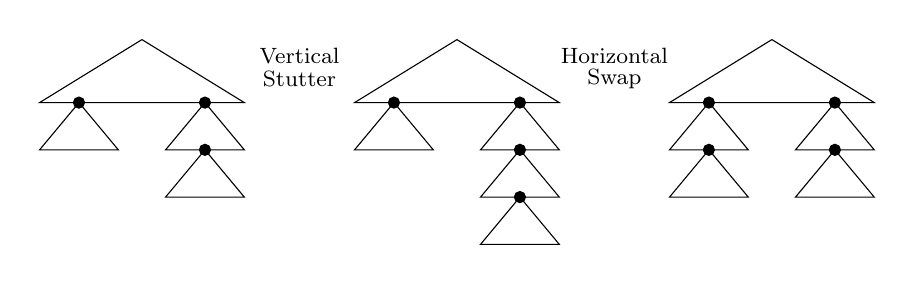
\begin{tikzpicture}

\draw (2.5,2) -- (1.2,1.2) -- (3.8,1.2) -- (2.5,2);

\draw (1.7,1.2) -- (1.2,0.6) -- (2.2,0.6) -- (1.7,1.2);
\node[dot] at (1.7,1.2) {};
\node[bag] at (1.7,0.8) {};
\node[bag] at (1.4,1.0) {};

\draw (3.3,1.2) -- (2.8,0.6) -- (3.8,0.6) -- (3.3,1.2);
\node[dot] at (3.3,1.2) {};
\draw (3.3,0.6) -- (2.8,0) -- (3.8,0) -- (3.3,0.6);
\node[dot] at (3.3,0.6) {};

\node[bag] at (3.3,0.8) {};
\node[bag] at (3.3,0.2) {};
\node[bag] at (3.0,1.0) {};
\node[bag] at (3.0,0.4) {};



\node[bag] at (4.5,1.2) {};
\node[bag] at (4.5,1.8) {\footnotesize Vertical};
\node[bag] at (4.5,1.5) {\footnotesize Stutter};

\draw (6.5,2) -- (5.2,1.2) -- (7.8,1.2) -- (6.5,2);

\draw (5.7,1.2) -- (5.2,0.6) -- (6.2,0.6) -- (5.7,1.2);
\node[dot] at (5.7,1.2) {};
\node[bag] at (5.7,0.8) {};
\node[bag] at (5.4,1.0) {};


\draw (7.3,1.2) -- (6.8,0.6) -- (7.8,0.6) -- (7.3,1.2);
\node[dot] at (7.3,1.2) {};
\draw (7.3,0.6) -- (6.8,0) -- (7.8,0) -- (7.3,0.6);
\node[dot] at (7.3,0.6) {};
\draw (7.3,0) -- (6.8,-0.6) -- (7.8,-0.6) -- (7.3,0);
\node[dot] at (7.3,0) {};

\node[bag] at (7.3,0.8) {};
\node[bag] at (7.3,0.2) {};
\node[bag] at (7.3,-0.4) {};
\node[bag] at (7.0,1.0) {};
\node[bag] at (7.0,-0.2) {};


\node[bag] at (8.5,1.2) {};
\node[bag] at (8.5,1.8) {\footnotesize Horizontal};
\node[bag] at (8.5,1.5) {\footnotesize Swap};


\draw (10.5,2) -- (9.2,1.2) -- (11.8,1.2) -- (10.5,2);

\draw (9.7,1.2) -- (9.2,0.6) -- (10.2,0.6) -- (9.7,1.2);
\node[dot] at (9.7,1.2) {};
\draw (9.7,0.6) -- (9.2,0) -- (10.2,0) -- (9.7,0.6);
\node[dot] at (9.7,0.6) {};

\node[bag] at (9.7,0.8) {};
\node[bag] at (9.7,0.2) {};
\node[bag] at (9.4,1.0) {};

\draw (11.3,1.2) -- (10.8,0.6) -- (11.8,0.6) -- (11.3,1.2);
\node[dot] at (11.3,1.2) {};
\draw (11.3,0.6) -- (10.8,0) -- (11.8,0) -- (11.3,0.6);
\node[dot] at (11.3,0.6) {};

\node[bag] at (11.3,0.8) {};
\node[bag] at (11.3,0.2) {};
\node[bag] at (11.0,1.0) {};

\end{tikzpicture}
\end{center}


\item If  is an ancestor of , let  and notice that . Since  and  have the
  same \ktype, we use -guarded horizontal swap followed by a -guarded vertical
  stutter to delete the copy of  (see the picture below). The resulting tree is
   as desired.


\begin{center}
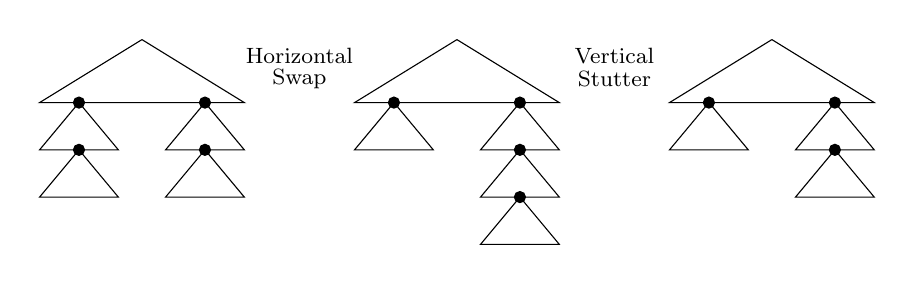
\begin{tikzpicture}


\draw (2.5,2) -- (1.2,1.2) -- (3.8,1.2) -- (2.5,2);

\draw (1.7,1.2) -- (1.2,0.6) -- (2.2,0.6) -- (1.7,1.2);
\node[dot] at (1.7,1.2) {};
\draw (1.7,0.6) -- (1.2,0) -- (2.2,0) -- (1.7,0.6);
\node[dot] at (1.7,0.6) {};

\node[bag] at (1.7,0.8) {};
\node[bag] at (1.7,0.2) {};
\node[bag] at (1.4,1.0) {};

\draw (3.3,1.2) -- (2.8,0.6) -- (3.8,0.6) -- (3.3,1.2);
\node[dot] at (3.3,1.2) {};
\draw (3.3,0.6) -- (2.8,0) -- (3.8,0) -- (3.3,0.6);
\node[dot] at (3.3,0.6) {};

\node[bag] at (3.3,0.8) {};
\node[bag] at (3.0,0.4) {};
\node[bag] at (3.3,0.2) {};
\node[bag] at (3.0,1.0) {};


\node[bag] at (4.5,1.2) {};
\node[bag] at (4.5,1.8) {\footnotesize Horizontal};
\node[bag] at (4.5,1.5) {\footnotesize Swap};

\draw (6.5,2) -- (5.2,1.2) -- (7.8,1.2) -- (6.5,2);

\draw (5.7,1.2) -- (5.2,0.6) -- (6.2,0.6) -- (5.7,1.2);
\node[dot] at (5.7,1.2) {};
\node[bag] at (5.7,0.8) {};
\node[bag] at (5.4,1.0) {};


\draw (7.3,1.2) -- (6.8,0.6) -- (7.8,0.6) -- (7.3,1.2);
\node[dot] at (7.3,1.2) {};
\draw (7.3,0.6) -- (6.8,0) -- (7.8,0) -- (7.3,0.6);
\node[dot] at (7.3,0.6) {};
\draw (7.3,0) -- (6.8,-0.6) -- (7.8,-0.6) -- (7.3,0);
\node[dot] at (7.3,0) {};

\node[bag] at (7.3,0.8) {};
\node[bag] at (7.3,0.2) {};
\node[bag] at (7.3,-0.4) {};
\node[bag] at (7.0,-0.2) {};


\node[bag] at (8.5,1.2) {};
\node[bag] at (8.5,1.8) {\footnotesize Vertical};
\node[bag] at (8.5,1.5) {\footnotesize Stutter};





\draw (10.5,2) -- (9.2,1.2) -- (11.8,1.2) -- (10.5,2);

\draw (9.7,1.2) -- (9.2,0.6) -- (10.2,0.6) -- (9.7,1.2);
\node[dot] at (9.7,1.2) {};
\node[bag] at (9.7,0.8) {};
\node[bag] at (9.4,1.0) {};

\draw (11.3,1.2) -- (10.8,0.6) -- (11.8,0.6) -- (11.3,1.2);
\node[dot] at (11.3,1.2) {};
\draw (11.3,0.6) -- (10.8,0) -- (11.8,0) -- (11.3,0.6);
\node[dot] at (11.3,0.6) {};

\node[bag] at (11.3,0.8) {};
\node[bag] at (11.3,0.2) {};
\node[bag] at (11.0,0.4) {};

\end{tikzpicture}
\end{center}


\item If  and  are not related by the descendant relation, then ,
  and  have the same \ktype and .
 We use -guarded horizontal transfer to replace \subtree{t''}{x} with
 \subtree{t''}{y} as depicted below.

\begin{center}
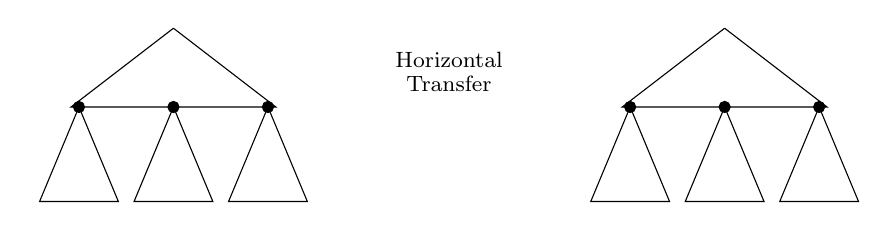
\begin{tikzpicture}

\draw (1.5,2.2) -- (0.2,1.2) -- (2.8,1.2) -- (1.5,2.2);

\draw (0.3,1.2) -- (-0.2,0) -- (0.8,0) -- (0.3,1.2);

\node[bag] at (0.3,0.4) {};
\node[bag] at (0,1.0) {};
\node[dot] at (0.3,1.2) {};


\draw (1.5,1.2) -- (1.0,0) -- (2.0,0) -- (1.5,1.2);

\node[bag] at (1.5,0.4) {};
\node[bag] at (1.2,1.0) {};
\node[dot] at (1.5,1.2) {};

\draw (2.7,1.2) -- (2.2,0) -- (3.2,0) -- (2.7,1.2);

\node[bag] at (2.7,0.4) {};
\node[bag] at (2.4,1.0) {};
\node[dot] at (2.7,1.2) {};


\node[bag] at (5.0,1.2) {};
\node[bag] at (5.0,1.8) {\footnotesize Horizontal};
\node[bag] at (5.0,1.5) {\footnotesize Transfer};


\draw (8.5,2.2) -- (7.2,1.2) -- (9.8,1.2) -- (8.5,2.2);

\draw (7.3,1.2) -- (6.8,0) -- (7.8,0) -- (7.3,1.2);

\node[bag] at (7.3,0.4) {};
\node[bag] at (7,1.0) {};
\node[dot] at (7.3,1.2) {};


\draw (8.5,1.2) -- (8.0,0) -- (9.0,0) -- (8.5,1.2);

\node[bag] at (8.5,0.4) {};
\node[bag] at (8.2,1.0) {};
\node[dot] at (8.5,1.2) {};

\draw (9.7,1.2) -- (9.2,0) -- (10.2,0) -- (9.7,1.2);

\node[bag] at (9.7,0.4) {};
\node[bag] at (9.4,1.0) {};
\node[dot] at (9.7,1.2) {};



\end{tikzpicture}
\end{center}


\end{enumerate}

\bigskip 

This concludes the case where  and  are not related by the descendant
relationship in . We are left with the case where  is a descendant of
 (recall that  is outside  and therefore not a descendant of ).
We reduce this problem to the previous case by considering two subcases:

\begin{iteMize}{}

\item If  are not related by the descendant relationship, we use a
  -guarded horizontal swap to replace  by  and vice versa. This
  reverses the roles of  and  and as  and  are not related by
  the descendant relationship and position  now has \type{(k+1)} 
  we can apply the previous case.

\begin{center}
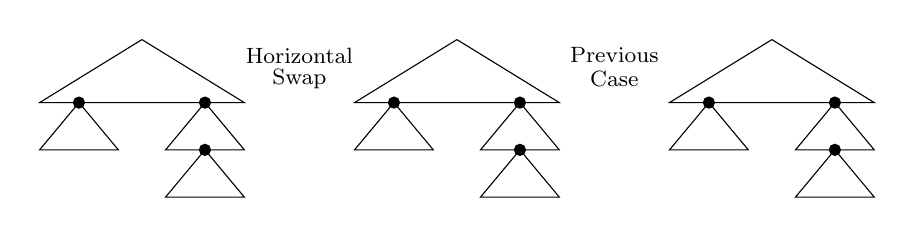
\begin{tikzpicture}

\draw (2.5,2) -- (1.2,1.2) -- (3.8,1.2) -- (2.5,2);


\draw (1.7,1.2) -- (1.2,0.6) -- (2.2,0.6) -- (1.7,1.2);
\node[dot] at (1.7,1.2) {};
\node[bag] at (1.7,0.8) {};
\node[bag] at (1.4,1.0) {};

\draw (3.3,1.2) -- (2.8,0.6) -- (3.8,0.6) -- (3.3,1.2);
\node[dot] at (3.3,1.2) {};
\draw (3.3,0.6) -- (2.8,0) -- (3.8,0) -- (3.3,0.6);
\node[dot] at (3.3,0.6) {};

\node[bag] at (3.3,0.2) {};
\node[bag] at (3.0,1.0) {};
\node[bag] at (3.0,0.4) {};



\node[bag] at (4.5,1.2) {};
\node[bag] at (4.5,1.8) {\footnotesize Horizontal};
\node[bag] at (4.5,1.5) {\footnotesize Swap};


\begin{scope}[xshift=4cm]


\draw (2.5,2) -- (1.2,1.2) -- (3.8,1.2) -- (2.5,2);


\draw (1.7,1.2) -- (1.2,0.6) -- (2.2,0.6) -- (1.7,1.2);
\node[dot] at (1.7,1.2) {};
\node[bag] at (1.7,0.8) {};
\node[bag] at (1.4,1.0) {};

\draw (3.3,1.2) -- (2.8,0.6) -- (3.8,0.6) -- (3.3,1.2);
\node[dot] at (3.3,1.2) {};
\draw (3.3,0.6) -- (2.8,0) -- (3.8,0) -- (3.3,0.6);
\node[dot] at (3.3,0.6) {};

\node[bag] at (3.3,0.2) {};
\node[bag] at (3.0,1.0) {};
\node[bag] at (3.0,0.4) {};

\end{scope}



\node[bag] at (8.5,1.2) {};
\node[bag] at (8.5,1.8) {\footnotesize Previous};
\node[bag] at (8.5,1.5) {\footnotesize Case};

\begin{scope}[xshift=8cm]


\draw (2.5,2) -- (1.2,1.2) -- (3.8,1.2) -- (2.5,2);


\draw (1.7,1.2) -- (1.2,0.6) -- (2.2,0.6) -- (1.7,1.2);
\node[dot] at (1.7,1.2) {};
\node[bag] at (1.7,0.8) {};
\node[bag] at (1.4,1.0) {};

\draw (3.3,1.2) -- (2.8,0.6) -- (3.8,0.6) -- (3.3,1.2);
\node[dot] at (3.3,1.2) {};
\draw (3.3,0.6) -- (2.8,0) -- (3.8,0) -- (3.3,0.6);
\node[dot] at (3.3,0.6) {};

\node[bag] at (3.3,0.2) {};
\node[bag] at (3.0,1.0) {};
\node[bag] at (3.0,0.4) {};

\end{scope}
\end{tikzpicture}
\end{center}

\item If  is an ancestor of both  and  we use -guarded vertical
  stutter to duplicate the context between  and . This introduces a new
  node  of type  that is not related to  by the descendant
  relationship and we are back in the previous case.

\end{iteMize}

\begin{center}
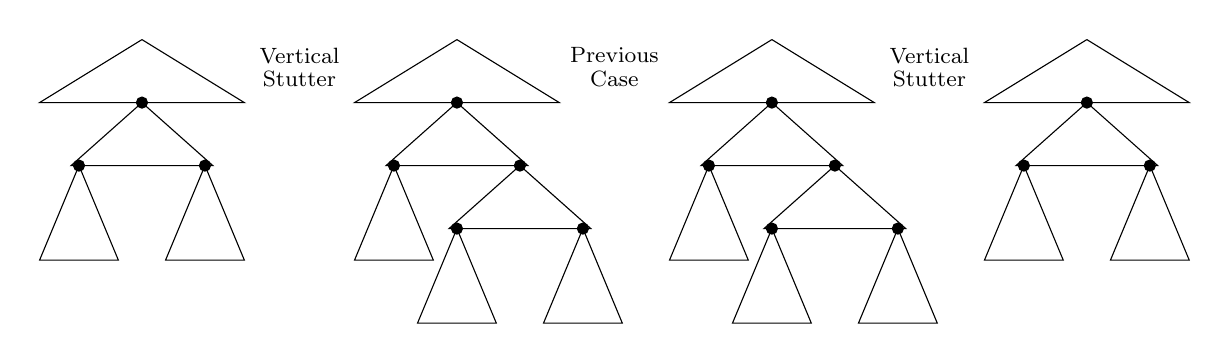
\begin{tikzpicture}

\draw (2.5,2) -- (1.2,1.2) -- (3.8,1.2) -- (2.5,2);

\draw (2.5,1.2) -- (1.6,0.4) -- (3.4,0.4) -- (2.5,1.2);
\node[dot] at (2.5,1.2) {};
\node[bag] at (2.5,0.7) {};
\node[bag] at (2.0,1.0) {};


\draw (1.7,0.4) -- (1.2,-0.8) -- (2.2,-0.8) -- (1.7,0.4);
\node[dot] at (1.7,0.4) {};
\node[bag] at (1.7,-0.4) {};
\node[bag] at (1.4,0.2) {};

\draw (3.3,0.4) -- (2.8,-0.8) -- (3.8,-0.8) -- (3.3,0.4);
\node[dot] at (3.3,0.4) {};


\node[bag] at (3.3,-0.4) {};
\node[bag] at (3.0,0.2) {};

\node[bag] at (4.5,1.2) {};
\node[bag] at (4.5,1.8) {\footnotesize Vertical};
\node[bag] at (4.5,1.5) {\footnotesize Stutter};


\begin{scope}[xshift=4cm]
\draw (2.5,2) -- (1.2,1.2) -- (3.8,1.2) -- (2.5,2);

\draw (2.5,1.2) -- (1.6,0.4) -- (3.4,0.4) -- (2.5,1.2);
\node[dot] at (2.5,1.2) {};
\node[bag] at (2.5,0.7) {};
\node[bag] at (2.0,1.0) {};


\draw (1.7,0.4) -- (1.2,-0.8) -- (2.2,-0.8) -- (1.7,0.4);
\node[dot] at (1.7,0.4) {};
\node[bag] at (1.7,-0.4) {};
\node[bag] at (1.4,0.2) {};

\end{scope}

\begin{scope}[xshift=4.8cm,yshift=-0.8cm]
\draw (2.5,1.2) -- (1.6,0.4) -- (3.4,0.4) -- (2.5,1.2);
\node[dot] at (2.5,1.2) {};
\node[bag] at (2.5,0.7) {};
\node[bag] at (2.0,1.0) {};


\draw (1.7,0.4) -- (1.2,-0.8) -- (2.2,-0.8) -- (1.7,0.4);
\node[dot] at (1.7,0.4) {};
\node[bag] at (1.7,-0.4) {};
\node[bag] at (1.4,0.2) {};

\draw (3.3,0.4) -- (2.8,-0.8) -- (3.8,-0.8) -- (3.3,0.4);
\node[dot] at (3.3,0.4) {};


\node[bag] at (3.3,-0.4) {};
\node[bag] at (3.0,0.2) {};

\end{scope}

\node[bag] at (8.5,1.2) {};
\node[bag] at (8.5,1.8) {\footnotesize Previous};
\node[bag] at (8.5,1.5) {\footnotesize Case};

\begin{scope}[xshift=8cm]
\draw (2.5,2) -- (1.2,1.2) -- (3.8,1.2) -- (2.5,2);

\draw (2.5,1.2) -- (1.6,0.4) -- (3.4,0.4) -- (2.5,1.2);
\node[dot] at (2.5,1.2) {};
\node[bag] at (2.5,0.7) {};
\node[bag] at (2.0,1.0) {};


\draw (1.7,0.4) -- (1.2,-0.8) -- (2.2,-0.8) -- (1.7,0.4);
\node[dot] at (1.7,0.4) {};
\node[bag] at (1.7,-0.4) {};
\node[bag] at (1.4,0.2) {};

\end{scope}

\begin{scope}[xshift=8.8cm,yshift=-0.8cm]
\draw (2.5,1.2) -- (1.6,0.4) -- (3.4,0.4) -- (2.5,1.2);
\node[dot] at (2.5,1.2) {};
\node[bag] at (2.5,0.7) {};
\node[bag] at (2.0,1.0) {};


\draw (1.7,0.4) -- (1.2,-0.8) -- (2.2,-0.8) -- (1.7,0.4);
\node[dot] at (1.7,0.4) {};
\node[bag] at (1.7,-0.4) {};
\node[bag] at (1.4,0.2) {};

\draw (3.3,0.4) -- (2.8,-0.8) -- (3.8,-0.8) -- (3.3,0.4);
\node[dot] at (3.3,0.4) {};


\node[bag] at (3.3,-0.4) {};
\node[bag] at (3.0,0.2) {};

\end{scope}

\node[bag] at (12.5,1.2) {};
\node[bag] at (12.5,1.8) {\footnotesize Vertical};
\node[bag] at (12.5,1.5) {\footnotesize Stutter};

\begin{scope}[xshift=12cm]
\draw (2.5,2) -- (1.2,1.2) -- (3.8,1.2) -- (2.5,2);

\draw (2.5,1.2) -- (1.6,0.4) -- (3.4,0.4) -- (2.5,1.2);
\node[dot] at (2.5,1.2) {};
\node[bag] at (2.5,0.7) {};
\node[bag] at (2.0,1.0) {};


\draw (1.7,0.4) -- (1.2,-0.8) -- (2.2,-0.8) -- (1.7,0.4);
\node[dot] at (1.7,0.4) {};
\node[bag] at (1.7,-0.4) {};
\node[bag] at (1.4,0.2) {};

\draw (3.3,0.4) -- (2.8,-0.8) -- (3.8,-0.8) -- (3.3,0.4);
\node[dot] at (3.3,0.4) {};


\node[bag] at (3.3,-0.4) {};
\node[bag] at (3.0,0.2) {};

\end{scope}

\end{tikzpicture}
\end{center}

\end{proof}

  We now turn to the proof of Lemma~\ref{claim-transfer-branch}. The proof is
  done by induction on the depth of . The idea is to replace   with 
  node by node.

  Assume first that  is of depth less than . Then because the \ktype of
  the roots of  and  are equal, we have  and the result follows.

  Assume now that  is of depth greater than . 

  Let  be the node of  corresponding to the root of . Let  be
  the \type{(k+1)} of the root of . We assume that  is a tree of the
  form . Notice that the \ktype of the roots of  and 
  are completely determined by . By hypothesis \lessblocks{s'}{D}{k+1},
  hence there exists a node  in  of type . We consider two
  cases depending on the relationship between  and .

\tikzstyle{arr} = [line width=4pt, ->]
\tikzstyle{bag}=[minimum size=20pt,inner sep=0pt]
\tikzstyle{inner}=[draw,circle,inner sep=0pt]
\tikzstyle{dot}=[draw,circle,fill,minimum size=4pt,inner sep=0pt]

\begin{iteMize}{}
\item If  is an ancestor of , let  be  and notice that  and
   have the same \ktype. This case is depicted below. Hence applying a -guarded vertical stutter we
  can duplicate  obtaining the tree . Because  is \ktame,  iff . Now the root of  in  is of type  and therefore of
  the form  where the roots of  and  have the same \ktype
  as respectively the roots of  and . By construction all the
  \types{(k+1)} of  and  already appear in  and hence we can apply
  the induction hypothesis to replace  by  and  by 
  without affecting membership in . Altogether this gives the desired
  result.
\begin{center}
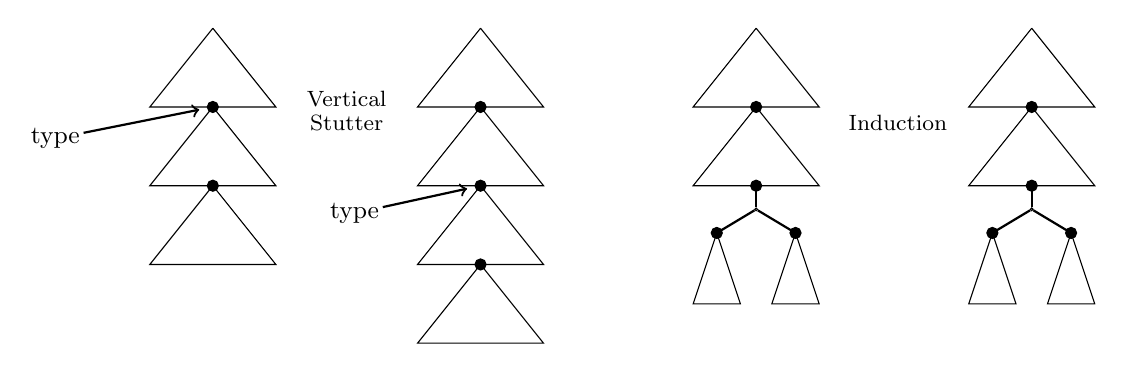
\begin{tikzpicture}

\draw (0.8,2) -- (0,1) -- (1.6,1) -- (0.8,2);
\draw (0.8,1) -- (0,0) -- (1.6,0) -- (0.8,1);
\draw (0.8,0) -- (0,-1) -- (1.6,-1) -- (0.8,0);

\node[dot] at (0.8,1) {};
\node[bag] at (1.2,0.8) {};
\node[dot] at (0.8,0) {};
\node[bag] at (1.2,-0.2) {};

\node[bag] at (0.8,0.4) {};
\node[bag] at (0.8,-0.6) {};

\node[bag] (type1) at (-1.2,0.6) {\small type };

\draw[->,shorten >=5pt, thick] (type1) -> (0.8,1);

\node[bag] at (2.5,1.1){\footnotesize Vertical};
\node[bag] at (2.5,0.8){\footnotesize Stutter};
\node[bag] at (2.5,0.5){};

\draw (4.2,2) -- (3.4,1) -- (5,1) -- (4.2,2);
\draw (4.2,1) -- (3.4,0) -- (5,0) -- (4.2,1);
\draw (4.2,0) -- (3.4,-1) -- (5,-1) -- (4.2,0);
\draw (4.2,-1) -- (3.4,-2) -- (5,-2) -- (4.2,-1);

\node[dot] at (4.2,1) {};
\node[bag] at (4.2,0.4) {};
\node[dot] at (4.2,0) {};
\node[bag] at (4.2,-0.6) {};
\node[dot] at (4.2,-1) {};
\node[bag] at (4.2,-1.6) {};

\node[bag] (type2) at (2.6,-0.35) {\small type };

\draw[->,shorten >=5pt, thick] (type2) -> (4.2,0);

\begin{scope}[xshift=3.5cm]

\node[bag] at (2.5,0.5){};

\draw (4.2,2) -- (3.4,1) -- (5,1) -- (4.2,2);
\draw (4.2,1) -- (3.4,0) -- (5,0) -- (4.2,1);

\draw (3.7,-0.6) -- (3.4,-1.5) -- (4.0,-1.5) -- (3.7,-0.6);
\draw (4.7,-0.6) -- (4.4,-1.5) -- (5,-1.5) -- (4.7,-0.6);

\node[bag] at (3.7,-1.2) {};
\node[bag] at (4.7,-1.2) {};

\node[dot] at (4.2,1) {};
\node[bag] at (4.2,0.4) {};
\node[dot] at (4.2,0) {};
\node[inner] (a) at (4.2,-0.3) {};

\node[dot] at (3.7,-0.6) {};
\node[dot] at (4.7,-0.6) {};

\draw[thick] (a) -- (3.7,-0.6);
\draw[thick] (a) -- (4.7,-0.6);
\draw[thick] (a) -- (4.2,0);


\end{scope}

\begin{scope}[xshift=7cm]

\node[bag] at (2.5,0.8){\footnotesize Induction};
\node[bag] at (2.5,0.5){};

\draw (4.2,2) -- (3.4,1) -- (5,1) -- (4.2,2);
\draw (4.2,1) -- (3.4,0) -- (5,0) -- (4.2,1);

\draw (3.7,-0.6) -- (3.4,-1.5) -- (4.0,-1.5) -- (3.7,-0.6);
\draw (4.7,-0.6) -- (4.4,-1.5) -- (5,-1.5) -- (4.7,-0.6);

\node[bag] at (3.7,-1.2) {};
\node[bag] at (4.7,-1.2) {};

\node[dot] at (4.2,1) {};
\node[bag] at (4.2,0.4) {};
\node[dot] at (4.2,0) {};
\node[inner] (a) at (4.2,-0.3) {};

\node[dot] at (3.7,-0.6) {};
\node[dot] at (4.7,-0.6) {};

\draw[thick] (a) -- (3.7,-0.6);
\draw[thick] (a) -- (4.7,-0.6);
\draw[thick] (a) -- (4.2,0);

\end{scope}

\end{tikzpicture}
\end{center}

\item Assume now that  and  are not related by the descendant
  relationship. This case is depicted below. Let  be the subtree of  rooted at .  By hypothesis
  all the \types{(k+1)} of  are already present in  and the roots of 
  and  have the same \ktype. Hence we can apply
  Claim~\ref{claim-transfer-enhanced} and we have  iff .
  Now the root of  is by construction of type . Hence  is
  of the form  where  and  have all their \types{(k+1)}
  appearing in  and their roots have the same \ktype as respectively
   and . Hence by induction  can be replaced by  and
   by  without affecting membership in . Altogether this gives
  the desired result.

\begin{center}
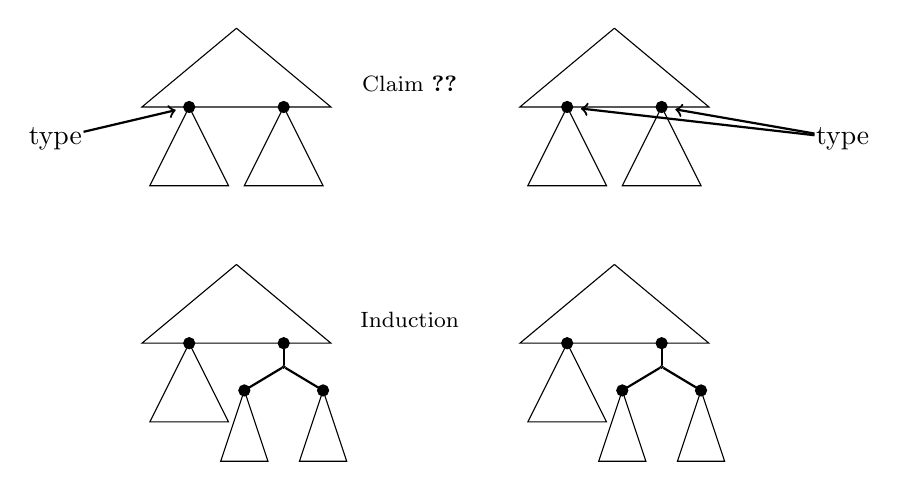
\begin{tikzpicture}

\draw (0.8,2) -- (-0.4,1) -- (2,1) -- (0.8,2);
\draw (0.2,1) -- (-0.3,0) -- (0.7,0) -- (0.2,1);
\draw (1.4,1) -- (0.9,0) -- (1.9,0) -- (1.4,1);

\node[dot] at (0.2,1) {};
\node[bag] at (0.5,0.8) {};
\node[dot] at (1.4,1) {};
\node[bag] at (1.7,0.8) {};

\node[bag] at (0.2,0.4) {};
\node[bag] at (1.4,0.4) {};

\node[bag] (type1) at (-1.5,0.6) {type };

\draw[->,shorten >=5pt, thick] (type1) -> (0.2,1);

\node[bag] at (3,1.3){\footnotesize Claim~\ref{claim-transfer-enhanced}};
\node[bag] at (3,1){};

\draw (5.6,2) -- (4.4,1) -- (6.8,1) -- (5.6,2);
\draw (5,1) -- (4.5,0) -- (5.5,0) -- (5,1);
\draw (6.2,1) -- (5.7,0) -- (6.7,0) -- (6.2,1);

\node[dot] at (5,1) {};
\node[bag] at (5.3,0.8) {};
\node[dot] at (6.2,1) {};
\node[bag] at (6.5,0.8) {};

\node[bag] at (5,0.4) {};
\node[bag] at (6.2,0.4) {};

\node[bag] (type2) at (8.5,0.6) {type };

\draw[->,shorten >=5pt, thick] (type2) -> (5,1);
\draw[->,shorten >=5pt, thick] (type2) -> (6.2,1);

\node[bag] at (5.6,-0.5){};



\begin{scope}[yshift=-3cm]

\draw (0.8,2) -- (-0.4,1) -- (2,1) -- (0.8,2);
\draw (0.2,1) -- (-0.3,0) -- (0.7,0) -- (0.2,1);


\node[dot] at (0.2,1) {};
\node[bag] at (0.5,0.8) {};
\node[dot] at (1.4,1) {};
\node[bag] at (1.7,0.8) {};

\node[bag] at (0.2,0.4) {};

\begin{scope} [xshift=-2.8cm,yshift=1cm]

\draw (3.7,-0.6) -- (3.4,-1.5) -- (4.0,-1.5) -- (3.7,-0.6);
\draw (4.7,-0.6) -- (4.4,-1.5) -- (5,-1.5) -- (4.7,-0.6);

\node[bag] at (3.7,-1.2) {};
\node[bag] at (4.7,-1.2) {};

\node[inner] (a) at (4.2,-0.3) {};

\node[dot] at (3.7,-0.6) {};
\node[dot] at (4.7,-0.6) {};

\draw[thick] (a) -- (3.7,-0.6);
\draw[thick] (a) -- (4.7,-0.6);
\draw[thick] (a) -- (4.2,0);
\end{scope}

\node[bag] at (3,1.3){\footnotesize Induction};
\node[bag] at (3,1){};

\draw (5.6,2) -- (4.4,1) -- (6.8,1) -- (5.6,2);
\draw (5,1) -- (4.5,0) -- (5.5,0) -- (5,1);

\node[dot] at (5,1) {};
\node[bag] at (5.3,0.8) {};
\node[dot] at (6.2,1) {};
\node[bag] at (6.5,0.8) {};

\node[bag] at (5,0.4) {};

\begin{scope} [xshift=2cm,yshift=1cm]

\draw (3.7,-0.6) -- (3.4,-1.5) -- (4.0,-1.5) -- (3.7,-0.6);
\draw (4.7,-0.6) -- (4.4,-1.5) -- (5,-1.5) -- (4.7,-0.6);

\node[bag] at (3.7,-1.2) {};
\node[bag] at (4.7,-1.2) {};

\node[inner] (a) at (4.2,-0.3) {};

\node[dot] at (3.7,-0.6) {};
\node[dot] at (4.7,-0.6) {};

\draw[thick] (a) -- (3.7,-0.6);
\draw[thick] (a) -- (4.7,-0.6);
\draw[thick] (a) -- (4.2,0);
\end{scope}
\end{scope}

\end{tikzpicture}
\end{center}
\end{iteMize}
\end{proof}

We now prove a similar result for \kloops.

\begin{lem}\label{lemma-insert-loop}
  Assume  is \ktame. Let  be a tree and  a node of  of \ktype
  . Let  be another tree such that \sameblocks{t}{t'}{k+1} and  be
  a \kloop of type  in . Consider the tree  constructed from 
  by inserting a copy of  at . Then  iff .
\end{lem}

\begin{proof} 

The proof is done in two steps. First we use the \ktame property
  of  to show that we can insert a \kloop  at  in  such that the
  principal path of  is the same as the principal path of . By this we
  mean that there is a bijection from the principal path of  to the
  principal path of  that preserves the child relation and \types{(k+1)}.  In a second step we
  replace one by one the subtrees hanging from the principal path of  with
  the corresponding subtrees in .

  First some terminology. Given two nodes  of some tree , we say that
   is a {\bf l}-ancestor of  if  is a descendant of the left child of
  . Similarly we define {\bf r}-ancestorship.

  Consider the context  occurring in . Let  be the
  nodes of  on the principal path of  and  be
  their respective \type{(k+1)}. For , set  to {\bf l}
  if  is a left child of  and {\bf r} otherwise.

  From  we construct using -guarded swaps and -vertical stutters a
  tree  such that there is a sequence of nodes  in 
  with for all ,  is of type  and  is an
  -ancestor of . The tree  is constructed by induction on
   (note that this step do not require that  is a \kloop).
  If  then this is a consequence of \sameblocks{t}{t'}{k+1} that one
  can find in  a node of type .  Consider now the case . By
  induction we have constructed from  a tree  such that
   is an appropriate sequence in .  By symmetry it is
  enough to consider the case where  is the left child of .
  Because all -guarded operations preserve \types{(k+1)}, we have
  \sameblocks{t}{t'_1}{k+1} and hence there is a node  of  of type
  . If  is a {\bf l}-ancestor of  then we are done.
  Otherwise consider the left child  of  and notice that because 
  is a child of  and  has the same \type{(k+1)} as
   then ,  and  have the same \ktype.

  We know that  is not a descendant of . There are two cases. If  and 
  are not related by the descendant relationship then by -guarded swaps we
  can replace the subtree rooted in  by the subtree rooted in  and we
  are done. If  is an ancestor of  then the context between  and 
  is a \kloop and we can use -guarded vertical stutter to duplicate
  it. This places a node having the same \type{(k+1)} as  as the left child of  and we are done.

  \noindent This concludes the construction of . From  we construct using
  -guarded swaps and -guarded vertical stutter a tree  such that
  there is a path  in  with  is of type 
  for all .

  Consider the sequence  obtained in  from the previous
  step. Recall that the \ktype of  is the same as the \ktype of .
  Hence using -guarded vertical stutter we can duplicate in  the
  context rooted in  and whose port is . Let  the resulting
  tree. We thus have two copies of the sequence  that we denote
  by the \emph{top copy} and the \emph{bottom copy}. Assume  is not a
  child of . By symmetry it is enough to consider the case where
   is a {\bf l}-ancestor of . Notice then that the context
  between the left child of  and  is a \kloop. Using -guarded
  vertical swap (see Figure~\ref{figure-construct-t2}) we can move the top copy
  of this context next to its bottom copy. Using -guarded vertical stutter
  this extra copy can be removed. We are left with an instance of the initial
  sequence in the bottom copy, while in the top one  is a child of
  .  This construction is depicted in
  figure~\ref{figure-construct-t2}.

\tikzstyle{arr} = [line width=4pt, ->]
\tikzstyle{bag}=[minimum size=20pt,inner sep=0pt]
\tikzstyle{dot}=[draw,circle,fill,minimum size=4pt,inner sep=0pt]

\begin{figure}
\begin{center}
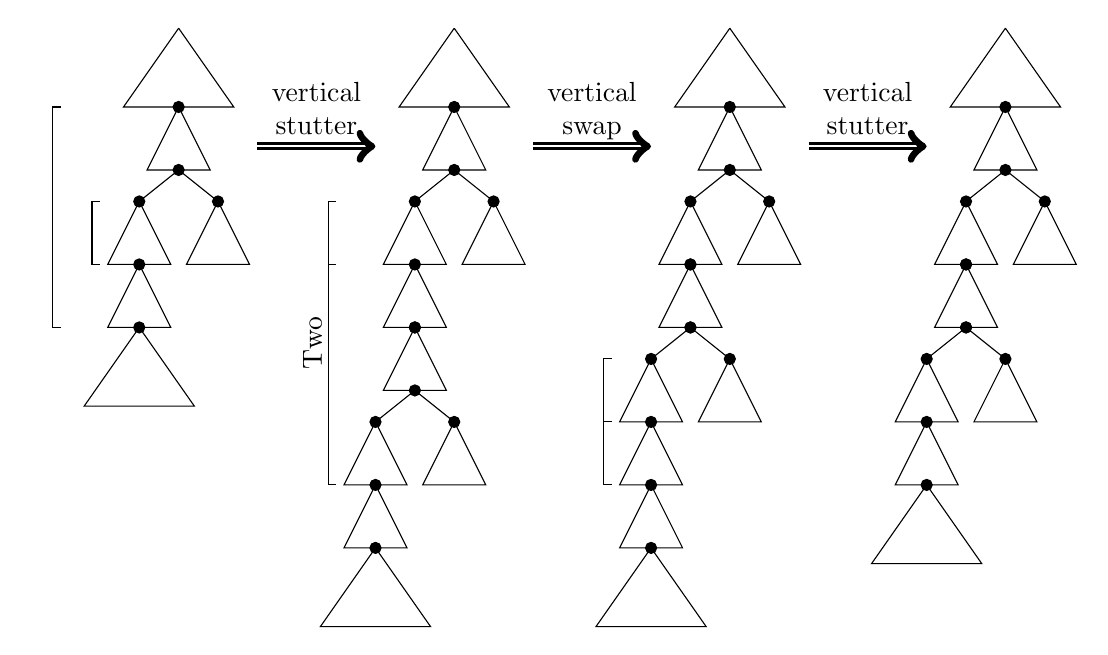
\begin{tikzpicture}




\draw (1.5,9.5) -- (0.8,8.5) -- (2.2,8.5) -- (1.5,9.5);

\draw (1.5,8.5) -- (1.1,7.7) -- (1.9,7.7) -- (1.5,8.5);

\draw (1.0,7.3) -- (1.4,6.5) -- (0.6,6.5) -- (1.0,7.3);
\draw (2.0,7.3) -- (2.4,6.5) -- (1.6,6.5) -- (2.0,7.3);

\draw (1.0,6.5) -- (1.4,5.7) -- (0.6,5.7) -- (1.0,6.5);

\draw (1.0,5.7) -- (1.7,4.7) -- (0.3,4.7) -- (1.0,5.7);

\node[dot] at (1.5,8.5) {};
\node[dot] at (1.5,7.7) {};
\node[dot] at (1.0,7.3) {};
\node[dot] at (2.0,7.3) {};
\node[dot] at (1.0,6.5) {};
\node[dot] at (1.0,5.7) {};

\draw (1.5,7.7) -- (1.0,7.3);
\draw (1.5,7.7) -- (2.0,7.3);


\node[bag] at (1.9,8.35) {};
\node[bag] at (2.1,7.55) {};

\node[bag] at (1.4,6.35) {};
\node[bag] at (1.4,5.55) {};


\node[bag] at (1.0,6.8) {};
\node[bag] at (1.5,8.0) {};
\node[bag] at (1.0,6.0) {};


\draw (0.5,7.3) -- (0.4,7.3) -- (0.4,6.5) -- (0.5,6.5);

\draw (0.0,8.5) -- (-0.1,8.5) -- (-0.1,5.7) -- (0.0,5.7);

\node[rotate=90] at (0.2,6.9) {\kloop};


\node[rotate=90] at (-0.3,7.1) {\kloop };



\draw[double,->,very thick] (2.5,8.0) to node[bag,sloped,above] {\begin{tabular}{c}vertical\\stutter\end{tabular}} (4.0,8.0);





\begin{scope}[xshift=3.5cm]
\draw (1.5,9.5) -- (0.8,8.5) -- (2.2,8.5) -- (1.5,9.5);

\draw (1.5,8.5) -- (1.1,7.7) -- (1.9,7.7) -- (1.5,8.5);

\draw (1.0,7.3) -- (1.4,6.5) -- (0.6,6.5) -- (1.0,7.3);
\draw (2.0,7.3) -- (2.4,6.5) -- (1.6,6.5) -- (2.0,7.3);

\draw (1.0,6.5) -- (1.4,5.7) -- (0.6,5.7) -- (1.0,6.5);

\node[dot] at (1.5,8.5) {};
\node[dot] at (1.5,7.7) {};
\node[dot] at (1.0,7.3) {};
\node[dot] at (2.0,7.3) {};
\node[dot] at (1.0,6.5) {};
\node[dot] at (1.0,5.7) {};

\draw (1.5,7.7) -- (1.0,7.3);
\draw (1.5,7.7) -- (2.0,7.3);


\node[bag] at (1.9,8.35) {};
\node[bag] at (2.1,7.55) {};

\node[bag] at (1.4,6.35) {};
\node[bag] at (1.4,5.55) {};


\node[bag] at (1.0,6.8) {};
\node[bag] at (1.5,8.0) {};
\node[bag] at (1.0,6.0) {};


\begin{scope}[xshift=-0.5cm,yshift=-2.8cm]


\draw (1.5,8.5) -- (1.1,7.7) -- (1.9,7.7) -- (1.5,8.5);

\draw (1.0,7.3) -- (1.4,6.5) -- (0.6,6.5) -- (1.0,7.3);
\draw (2.0,7.3) -- (2.4,6.5) -- (1.6,6.5) -- (2.0,7.3);

\draw (1.0,6.5) -- (1.4,5.7) -- (0.6,5.7) -- (1.0,6.5);

\draw (1.0,5.7) -- (1.7,4.7) -- (0.3,4.7) -- (1.0,5.7);

\node[dot] at (1.5,8.5) {};
\node[dot] at (1.5,7.7) {};
\node[dot] at (1.0,7.3) {};
\node[dot] at (2.0,7.3) {};
\node[dot] at (1.0,6.5) {};
\node[dot] at (1.0,5.7) {};

\draw (1.5,7.7) -- (1.0,7.3);
\draw (1.5,7.7) -- (2.0,7.3);





\node[bag] at (1.0,6.8) {};
\node[bag] at (1.5,8.0) {};
\node[bag] at (1.0,6.0) {};



\end{scope}
\draw (0.0,7.3) -- (-0.1,7.3) -- (-0.1,3.7) -- (0.0,3.7);
\draw (0.0,6.5) -- (-0.1,6.5);

\node[rotate=90] at (-0.3,5.5) {Two \kloops};


\draw[double,->,very thick] (2.5,8.0) to node[bag,sloped,above] {\begin{tabular}{c}vertical\\swap\end{tabular}} (4.0,8.0);

\end{scope}













\begin{scope}[xshift=7.0cm]
\draw (1.5,9.5) -- (0.8,8.5) -- (2.2,8.5) -- (1.5,9.5);

\draw (1.5,8.5) -- (1.1,7.7) -- (1.9,7.7) -- (1.5,8.5);

\draw (1.0,7.3) -- (1.4,6.5) -- (0.6,6.5) -- (1.0,7.3);
\draw (2.0,7.3) -- (2.4,6.5) -- (1.6,6.5) -- (2.0,7.3);



\node[dot] at (1.5,8.5) {};
\node[dot] at (1.5,7.7) {};
\node[dot] at (1.0,7.3) {};
\node[dot] at (2.0,7.3) {};
\node[dot] at (1.0,6.5) {};
\node[dot] at (1.0,5.7) {};

\draw (1.5,7.7) -- (1.0,7.3);
\draw (1.5,7.7) -- (2.0,7.3);


\node[bag] at (1.9,8.35) {};
\node[bag] at (2.1,7.55) {};

\node[bag] at (1.4,7.15) {};
\node[bag] at (1.4,6.35) {};

\node[bag] at (1.5,8.0) {};
\node[bag] at (1.0,6.8) {};


\begin{scope}[xshift=-0.5cm,yshift=-2.0cm]


\draw (1.5,8.5) -- (1.1,7.7) -- (1.9,7.7) -- (1.5,8.5);

\draw (1.0,7.3) -- (1.4,6.5) -- (0.6,6.5) -- (1.0,7.3);
\draw (2.0,7.3) -- (2.4,6.5) -- (1.6,6.5) -- (2.0,7.3);

\draw (1.0,6.5) -- (1.4,5.7) -- (0.6,5.7) -- (1.0,6.5);
\draw (1.0,5.7) -- (1.4,4.9) -- (0.6,4.9) -- (1.0,5.7);


\draw (1.0,4.9) -- (1.7,3.9) -- (0.3,3.9) -- (1.0,4.9);

\node[dot] at (1.5,8.5) {};
\node[dot] at (1.5,7.7) {};
\node[dot] at (1.0,7.3) {};
\node[dot] at (2.0,7.3) {};
\node[dot] at (1.0,6.5) {};
\node[dot] at (1.0,5.7) {};
\node[dot] at (1.0,4.9) {};

\draw (1.5,7.7) -- (1.0,7.3);
\draw (1.5,7.7) -- (2.0,7.3);


\draw (0.5,7.3) -- (0.4,7.3) -- (0.4,5.7) -- (0.5,5.7);
\draw (0.5,6.5) -- (0.4,6.5);


\node[bag] at (1.0,6.8) {};
\node[bag] at (1.5,8.0) {};
\node[bag] at (1.0,6.0) {};
\node[bag] at (1.0,5.2) {};



\end{scope}

\draw[double,->,very thick] (2.5,8.0) to node[bag,sloped,above] {\begin{tabular}{c}vertical\\stutter\end{tabular}} (4.0,8.0);
\end{scope}



















\begin{scope}[xshift=10.5cm]
\draw (1.5,9.5) -- (0.8,8.5) -- (2.2,8.5) -- (1.5,9.5);

\draw (1.5,8.5) -- (1.1,7.7) -- (1.9,7.7) -- (1.5,8.5);

\draw (1.0,7.3) -- (1.4,6.5) -- (0.6,6.5) -- (1.0,7.3);
\draw (2.0,7.3) -- (2.4,6.5) -- (1.6,6.5) -- (2.0,7.3);



\node[dot] at (1.5,8.5) {};
\node[dot] at (1.5,7.7) {};
\node[dot] at (1.0,7.3) {};
\node[dot] at (2.0,7.3) {};
\node[dot] at (1.0,6.5) {};
\node[dot] at (1.0,5.7) {};

\draw (1.5,7.7) -- (1.0,7.3);
\draw (1.5,7.7) -- (2.0,7.3);


\node[bag] at (1.9,8.35) {};
\node[bag] at (2.1,7.55) {};

\node[bag] at (1.4,7.15) {};
\node[bag] at (1.4,6.35) {};

\node[bag] at (1.5,8.0) {};
\node[bag] at (1.0,6.8) {};


\begin{scope}[xshift=-0.5cm,yshift=-2.0cm]


\draw (1.5,8.5) -- (1.1,7.7) -- (1.9,7.7) -- (1.5,8.5);

\draw (1.0,7.3) -- (1.4,6.5) -- (0.6,6.5) -- (1.0,7.3);
\draw (2.0,7.3) -- (2.4,6.5) -- (1.6,6.5) -- (2.0,7.3);

\draw (1.0,6.5) -- (1.4,5.7) -- (0.6,5.7) -- (1.0,6.5);


\draw (1.0,5.7) -- (1.7,4.7) -- (0.3,4.7) -- (1.0,5.7);

\node[dot] at (1.5,8.5) {};
\node[dot] at (1.5,7.7) {};
\node[dot] at (1.0,7.3) {};
\node[dot] at (2.0,7.3) {};
\node[dot] at (1.0,6.5) {};
\node[dot] at (1.0,5.7) {};

\draw (1.5,7.7) -- (1.0,7.3);
\draw (1.5,7.7) -- (2.0,7.3);





\node[bag] at (1.0,6.8) {};
\node[bag] at (1.5,8.0) {};
\node[bag] at (1.0,6.0) {};



\end{scope}


\end{scope}















\end{tikzpicture}
\end{center}
\caption{The construction of , eliminating the context  between
   and }\label{figure-construct-t2}
\end{figure}

 Repeating this argument yields the desired
  tree .
 
Consider now the context . It is a loop of \ktype . Let
 be the tree constructed from  by inserting  at . 

\begin{claim} \label{claim-reverse-swaps}
 iff .
\end{claim}

\begin{proof}
  Consider the sequence of -guarded swaps and -guarded vertical stutter
  that was used in order to obtain  from . Because  is \ktame,  iff .

  We can easily identify the nodes of  with the nodes of  outside of
  . Consider the same sequence of -guarded operations applied to .
  Observe that this yields a tree  corresponding to  with possibly several
  extra copies of . As  is a \kloop, each of the roots and the ports of these
  extra copies have the same \ktype. Hence, using appropriate vertical -swaps or
  appropriate horizontal -swaps, depending on whether two copies are related or
  not by the descendant relation, they can be brought together. Two examples of
  such operation is given in Figure~\ref{figure-elim-loops}.





\begin{figure}
\begin{center}
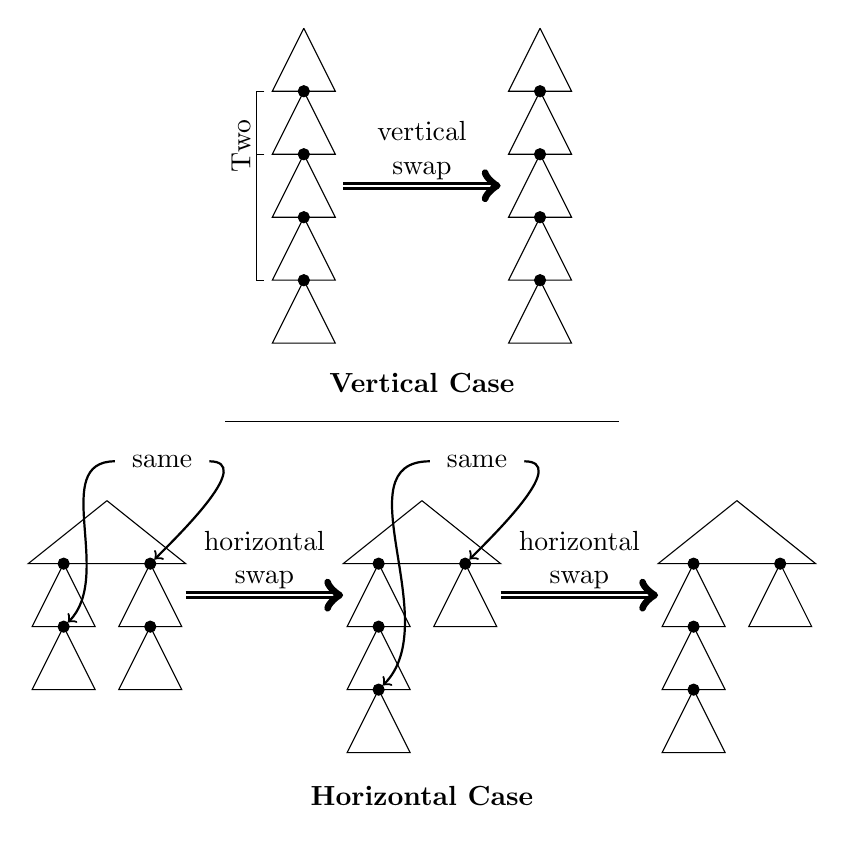
\begin{tikzpicture}




\draw (1.5,8.5) -- (1.1,7.7) -- (1.9,7.7) -- (1.5,8.5);
\draw (1.5,7.7) -- (1.1,6.9) -- (1.9,6.9) -- (1.5,7.7);
\draw (1.5,6.9) -- (1.1,6.1) -- (1.9,6.1) -- (1.5,6.9);
\draw (1.5,6.1) -- (1.1,5.3) -- (1.9,5.3) -- (1.5,6.1);
\draw (1.5,5.3) -- (1.1,4.5) -- (1.9,4.5) -- (1.5,5.3);


\node[dot] at (1.5,7.7) {};
\node[dot] at (1.5,6.9) {};
\node[dot] at (1.5,6.1) {};
\node[dot] at (1.5,5.3) {};

\node[bag] at (1.5,8.0) {};
\node[bag] at (1.5,7.2) {};
\node[bag] at (1.5,6.4) {};
\node[bag] at (1.5,5.6) {};
\node[bag] at (1.5,4.8) {};


\draw (1.0,7.7) -- (0.9,7.7) -- (0.9,5.3) -- (1.0,5.3);
\draw (1.0,6.9) -- (0.9,6.9);

\node[rotate=90] at (0.7,7.0) {Two \kloops};






\draw[double,->,very thick] (2.0,6.5) to node[bag,sloped,above] {\begin{tabular}{c}vertical\\swap\end{tabular}} (4.0,6.5);







\begin{scope}[xshift=3cm]
\draw (1.5,8.5) -- (1.1,7.7) -- (1.9,7.7) -- (1.5,8.5);
\draw (1.5,7.7) -- (1.1,6.9) -- (1.9,6.9) -- (1.5,7.7);
\draw (1.5,6.9) -- (1.1,6.1) -- (1.9,6.1) -- (1.5,6.9);
\draw (1.5,6.1) -- (1.1,5.3) -- (1.9,5.3) -- (1.5,6.1);
\draw (1.5,5.3) -- (1.1,4.5) -- (1.9,4.5) -- (1.5,5.3);


\node[dot] at (1.5,7.7) {};
\node[dot] at (1.5,6.9) {};
\node[dot] at (1.5,6.1) {};
\node[dot] at (1.5,5.3) {};

\node[bag] at (1.5,8.0) {};
\node[bag] at (1.5,7.2) {};
\node[bag] at (1.5,6.4) {};
\node[bag] at (1.5,5.6) {};
\node[bag] at (1.5,4.8) {};

\end{scope}

\node[bag] at (3.0,4.0) {\bf Vertical Case};

\draw (0.5,3.5) -- (5.5,3.5);


\begin{scope}[xshift=-2.5cm,yshift=-1cm]

\draw (1.5,3.5) -- (0.5,2.7) -- (2.5,2.7) -- (1.5,3.5);

\draw (0.95,2.7) -- (0.55,1.9) -- (1.35,1.9) -- (0.95,2.7);
\draw (0.95,1.9) -- (0.55,1.1) -- (1.35,1.1) -- (0.95,1.9);

\draw (2.05,2.7) -- (1.65,1.9) -- (2.45,1.9) -- (2.05,2.7);
\draw (2.05,1.9) -- (1.65,1.1) -- (2.45,1.1) -- (2.05,1.9);


\node[dot] at (0.95,2.7) {};
\node[dot] (s1) at (0.95,1.9) {};
\node[dot] (s2) at (2.05,2.7) {};
\node[dot] at (2.05,1.9) {};

\node[bag] at (0.95,2.2) {};
\node[bag] at (0.95,1.4) {};
\node[bag] at (2.05,2.2) {};
\node[bag] at (2.05,1.4) {};

\node[bag] (id) at (2.2,4.0) {\begin{tabular}{c}same\\ \ktype \end{tabular}};

\draw[->,thick] (id) to [out=180,in=45] (s1);
\draw[->,thick] (id) to [out=0,in=45] (s2);

\draw[double,->,very thick] (2.5,2.3) to node[bag,sloped,above] {\begin{tabular}{c}horizontal\\swap\end{tabular}} (4.5,2.3);


\end{scope}

\begin{scope}[xshift=1.5cm,yshift=-1cm]

\draw (1.5,3.5) -- (0.5,2.7) -- (2.5,2.7) -- (1.5,3.5);

\draw (0.95,2.7) -- (0.55,1.9) -- (1.35,1.9) -- (0.95,2.7);
\draw (0.95,1.9) -- (0.55,1.1) -- (1.35,1.1) -- (0.95,1.9);
\draw (0.95,1.1) -- (0.55,0.3) -- (1.35,0.3) -- (0.95,1.1);

\draw (2.05,2.7) -- (1.65,1.9) -- (2.45,1.9) -- (2.05,2.7);



\node[dot] at (0.95,2.7) {};
\node[dot] at (0.95,1.9) {};
\node[dot] (s2) at (2.05,2.7) {};
\node[dot] (s1) at (0.95,1.1) {};

\node[bag] at (0.95,2.2) {};
\node[bag] at (0.95,1.4) {};
\node[bag] at (2.05,2.2) {};
\node[bag] at (0.95,0.6) {};

\node[bag] (id) at (2.2,4.0) {\begin{tabular}{c}same\\ \ktype \end{tabular}};

\draw[->,thick] (id) to [out=180,in=45] (s1);
\draw[->,thick] (id) to [out=0,in=45] (s2);


\draw[double,->,very thick] (2.5,2.3) to node[bag,sloped,above] {\begin{tabular}{c}horizontal\\swap\end{tabular}} (4.5,2.3);


\end{scope}

\begin{scope}[xshift=5.5cm,yshift=-1cm]

\draw (1.5,3.5) -- (0.5,2.7) -- (2.5,2.7) -- (1.5,3.5);

\draw (0.95,2.7) -- (0.55,1.9) -- (1.35,1.9) -- (0.95,2.7);
\draw (0.95,1.9) -- (0.55,1.1) -- (1.35,1.1) -- (0.95,1.9);
\draw (0.95,1.1) -- (0.55,0.3) -- (1.35,0.3) -- (0.95,1.1);

\draw (2.05,2.7) -- (1.65,1.9) -- (2.45,1.9) -- (2.05,2.7);



\node[dot] at (0.95,2.7) {};
\node[dot] at (0.95,1.9) {};
\node[dot] at (2.05,2.7) {};
\node[dot] at (0.95,1.1) {};

\node[bag] at (0.95,2.2) {};
\node[bag] at (0.95,1.4) {};
\node[bag] at (2.05,2.2) {};
\node[bag] at (0.95,0.6) {};



\end{scope}

\node[bag] at (3.0,-1.25) {\bf Horizontal Case};

\end{tikzpicture}
\end{center}
\caption{Bringing copies of the \kloop  together in
Claim~\ref{claim-reverse-swaps}}\label{figure-elim-loops}
\end{figure}






Then, using -guarded vertical stutter all but one copy can be eliminated
resulting in . Hence  iff  and the claim is
proved. See figure \ref{figure-relat-t2}.
\end{proof}

\begin{figure}
\begin{center}
\psset{unit=.8cm}
\begin{pspicture}(8,6.6)

\rput(0.0,1.0){
\pspolygon(1.5,5.6)(0.2,3.3)(2.8,3.3)
\rput(1.5,4.3){}
}
\pspolygon(1.5,2.3)(0.2,0)(2.8,0)
\rput(1.5,1.0){}


\rput(0.0,1.0){
\rput(4.0,4.4){}
\rput(4.0,5.2){- guarded}
\rput(4.0,4.8){operations}
}

\rput(4.0,1.1){}
\rput(4.0,1.9){- guarded}
\rput(4.0,1.5){operations}



\rput(1.0,1.0){

\pspolygon(5.5,5.6)(4.2,3.3)(6.8,3.3)
\rput(5.5,4.3){}

}

\rput(1.0,0.0){
\pspolygon(5.5,2.3)(4.2,0)(6.8,0)
\rput(5.5,1.0){}

}

\rput(1.0,0.5){

\rput(5.5,2.8){\rotateleft{}}
\rput(6.8,3.2){deletion}
\rput(6.8,2.8){of extra}
\rput(6.8,2.4){copies of }

}

\end{pspicture}
\end{center}
\caption{Relation with }\label{figure-relat-t2}
\end{figure}


It remains to show that  iff . By construction of  we
have \lessblocks{C'}{t}{k+1}. Consider now a node  in the principal path
of . Let  be the subtree branching out the principal path of  at
 and  be the subtree branching out the principal path of  at
. By construction  and  are of \type{(k+1)} . Therefore
the roots of  and  have the same \ktype. Because
\lessblocks{C'}{t}{k+1} all the \types{(k+1)} of  already appear in the
part of  outside of . By hypothesis we also have \lessblocks{T_i}{t}{k+1}.
Hence we can apply Lemma~\ref{claim-transfer-branch} and replacing 
with  does not affect membership in . A repeated use of that
lemma eventually shows that  iff .
\end{proof}

\medskip

We return to the proof of Proposition~\ref{lemma-pumping}. Recall that
we have two trees  such that \sameblocks{t}{t'}{\kappa} for . For , we want to construct  such that:
 
\begin{enumerate}[(1)]
\item  iff 
\item  iff 
\item \sameblocks{T}{T'}{l}
\end{enumerate}



Recall that the number of \ktypes is . Therefore, by choice of , in
every branch of a \type{\kappa} one can find at least one \ktype that is repeated.
This provides many \kloops that can be used using Lemma~\ref{lemma-insert-loop}
for obtaining bigger types.

Take , we build  and  from  and  by inserting \kloops
in  and  without affecting their membership in  using
Lemma~\ref{lemma-insert-loop}.

  Let  be the set of \ktypes  such that
  there is a loop of \ktype  in  or in . For each  we
  fix a context  as follows. Because  there is a context
   in  or  that is a loop of \ktype . For each , we
  fix arbitrarily such a  and set  as ,  concatenations of the context . Notice that the path
  from the root of  to its port is then bigger than .

  We now describe the construction of  from . The construction of 
  from  is done similarly. The tree  is constructed by simultaneously inserting,
  for all , a copy of the context  at all nodes of  of type .

  We now show that  and  have the desired properties. 
  
  The first and second properties,  iff  and  iff
  , essentially follow from Lemma~\ref{lemma-insert-loop}. We only
  show that  iff , the second property is proved
  symmetrically. We view  as if it was constructed from  using a sequence
  of insertions of some context  for . We write
   the sequence of intermediate trees with  and . We
  call  the context inserted to get  from .  We show by
  induction on  that (i) \sameblocks{s_i}{t}{k+1} and (ii)  iff
  . This will imply  iff  as desired.  (i) is
  clear for . We show that for all  (i) implies (ii). Recall that 
  is the concatenation of  copies of a \kloop present either in  or in
  .  We suppose without generality that the \kloop is present in .  Let
   be the tree constructed from  by duplicating the \kloop 
  times. Hence  is a tree containing  and by construction
  \sameblocks{s}{t}{k+1}. Because \sameblocks{t}{t'}{\kappa} with  and \sameblocks{s_i}{t}{k+1} we have \sameblocks{s}{s_i}{k+1}. By
  Lemma~\ref{lemma-insert-loop} this implies that  iff . By construction we also have \sameblocks{s_{i+1}}{s_i}{k+1} and the
  induction step is proved.


We now show the third property:

  \begin{lem}\label{claim-sameblock}
    \sameblocks{T}{T'}{l}
  \end{lem}

\proof
  We need to show that \lessblocks{T}{T'}{l}, \lessblocks{T'}{T}{l} and that
  the roots of  and  have the same \type{l}. It will be convenient for
  proving this to view the nodes of  as the union of the nodes of  plus
  some nodes coming from the \kloops that were inserted. To do this more
  formally, if  is a node of  of \ktype not in , then  is
  identified with the corresponding node of . If  is a node of  whose
  \ktype is in  then  is identified in  with the port of the copy of
   that was inserted at node .  We start with the following claim.


  \begin{claim} \label{claim-identify-types} Take two nodes  in  and 
    in , such that  and  have the same \type{\kappa}. Let  and  be
    the corresponding nodes in  and . Then  and  have the same
    \type{l}.
\end{claim}


\begin{proof}
  Let  the \type{\kappa} of  and .  Consider a branch of  of
  length . By the choice of  we know that in this branch one
  can find two nodes  and  with the same \ktypes , with  an
  ancestor of  and such that the \ktype  of  is determined by
   ( is at distance  from the leaves of ). Hence  is
  in .  Note that because the \ktype of  is included in , the
  presence of a node of type  induces the presence of a node of type
   at the same relative position than . Hence a copy of  is
  inserted simultaneously at the same position relative to  and  during the
  construction of  and .  Because this is true for all branches of 
  and because all  have depth at least , then  and  have the
  same \type{l}.
\end{proof}

From claim~\ref{claim-identify-types} it follows that the roots of  and 
have the same \type{l}. By symmetry we only need to show that
\lessblocks{T}{T'}{l}. Let  be a node of  and  be its \type{l}. We
show that there exists  with type . We consider two cases:

\begin{iteMize}{}
\item  is not a node of a loop inserted during the construction of . Let
   be the corresponding position in  and let  be its \type{\kappa}. Since
  \sameblocks{t}{t'}{\kappa}, there is a node  of  of type . Let 
  be the node of  corresponding to . By
  Claim~\ref{claim-identify-types}  and  have the same \type{l}.

\item  is a node inside a copy of  inserted to construct . Let  be the
  node of  where this loop was inserted. Let  be the \type{\kappa} of  (the \ktype of
   is ).  Since \sameblocks{t}{t'}{\kappa}, there is a node  of  of
  type . Since ,  and  have the same \type{k}, a
  copy of  was also inserted in  at position  during the
  construction of . From Claim~\ref{claim-identify-types},  and
  , when viewed as nodes of  and  have the same \type{l}.  Let  be the node of  in the copy of
   inserted at  that corresponds to the position . Since  and
   are ancestors of  and  that have the same \type{l}, and since the
  context from  to  is the same as the context from  to , then  and  must have the same
  \type{l}.\qed
\end{iteMize}

\noindent This concludes the proof of Proposition~\ref{lemma-pumping}.
\end{proof}


